\subsection{Datenbank und Cloudspeicher}\label{datenbank und cloudspeicher}
Unsere Datenbank ist ein Firestore von Firebase. Firestore ist ein Cloud NOSQL Datenbanksystem. Die Daten werden in sogenannte Kollektionen und Dokumente eingeteilt. Dabei gehören zu jeder Kollektion Dokumente, in welchen die eigentlichen Daten gespeichert sind. Die Datenbank hat die folgenden Kollektionen und Dokumente.

\begin{figure}[h]
 \centering
 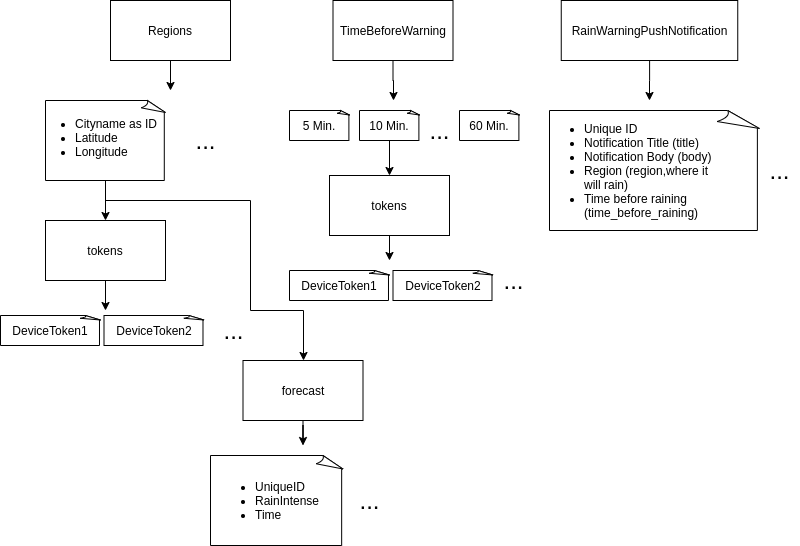
\includegraphics[width=0.6\textwidth,angle=0]{abb/firebase_aufbau}
 \caption[Datenbankarchitektur]{Der Aufbau der Kollektionen und Dokumente in der Firebase}
\label{fig:Beschreibung}
\end{figure}

Jedes Gerät besitzt einen einmaligen Device Token welcher in zwei Kollektionen gespeichert wird. Einmal in der Kollektion für einen bestimmten Zeitpunkt, und in der Kollektion der jeweiligen Region in der sich das Gerät befindet.
Alle fünf Minuten wird vom Server ein Dokument mit der neusten Regenvorhersage in die Kollektion Forecast der jeweiligen Region gepusht. Dieses Dokument enthält ein Feld mit der jeweiligen Regenintensität und ein Feld mit der Uhrzeit dieser Vorhersage. In den Einstellungen der App kann eingestellt werden wann die Regenwarnung als Push-Benachrichtigung gesendet werden soll. Dabei kann zwischen 5 und 60 Minuten im 5 Minutentakt jede Zeit ausgewählt werden. Je nachdem was der User einstellt, wird sein Devicetoken in eine andere Kollektion gespeichert. Dabei gibt es für jede einstellbare Zeit ein eigenes Dokument in der Kollektion TimeBeforeWarning. Wenn die Netze Regen vorhersagen wird vom Server ein Dokument in RainWarningPushNotification gepusht. Dieses Dokument wird von einer Cloud-Function (Siehe Kapitel Push Nachrichten) verwendet um die Push Benachrichtigungen an die richtigen Geräte zu senden.
Der Cloud Storage von Firebase wird verwendet um die PNGs mit der jeweiligen Vorhersage zu übertragen. Dabei pushed der Server gleichzeitig mit den Daten im Firestore auch ein PNG. Dieses PNG wird in der App angezeigt. 